\section{Application Interface}
\label{sec:app_interface}

The frontend is a single-page application arranged in a fixed-height two-panel layout that fills the browser viewport without scrolling at the page level.
Figure~\ref{fig:app_interface} shows the full interface.

\begin{figure}[H]
\centering
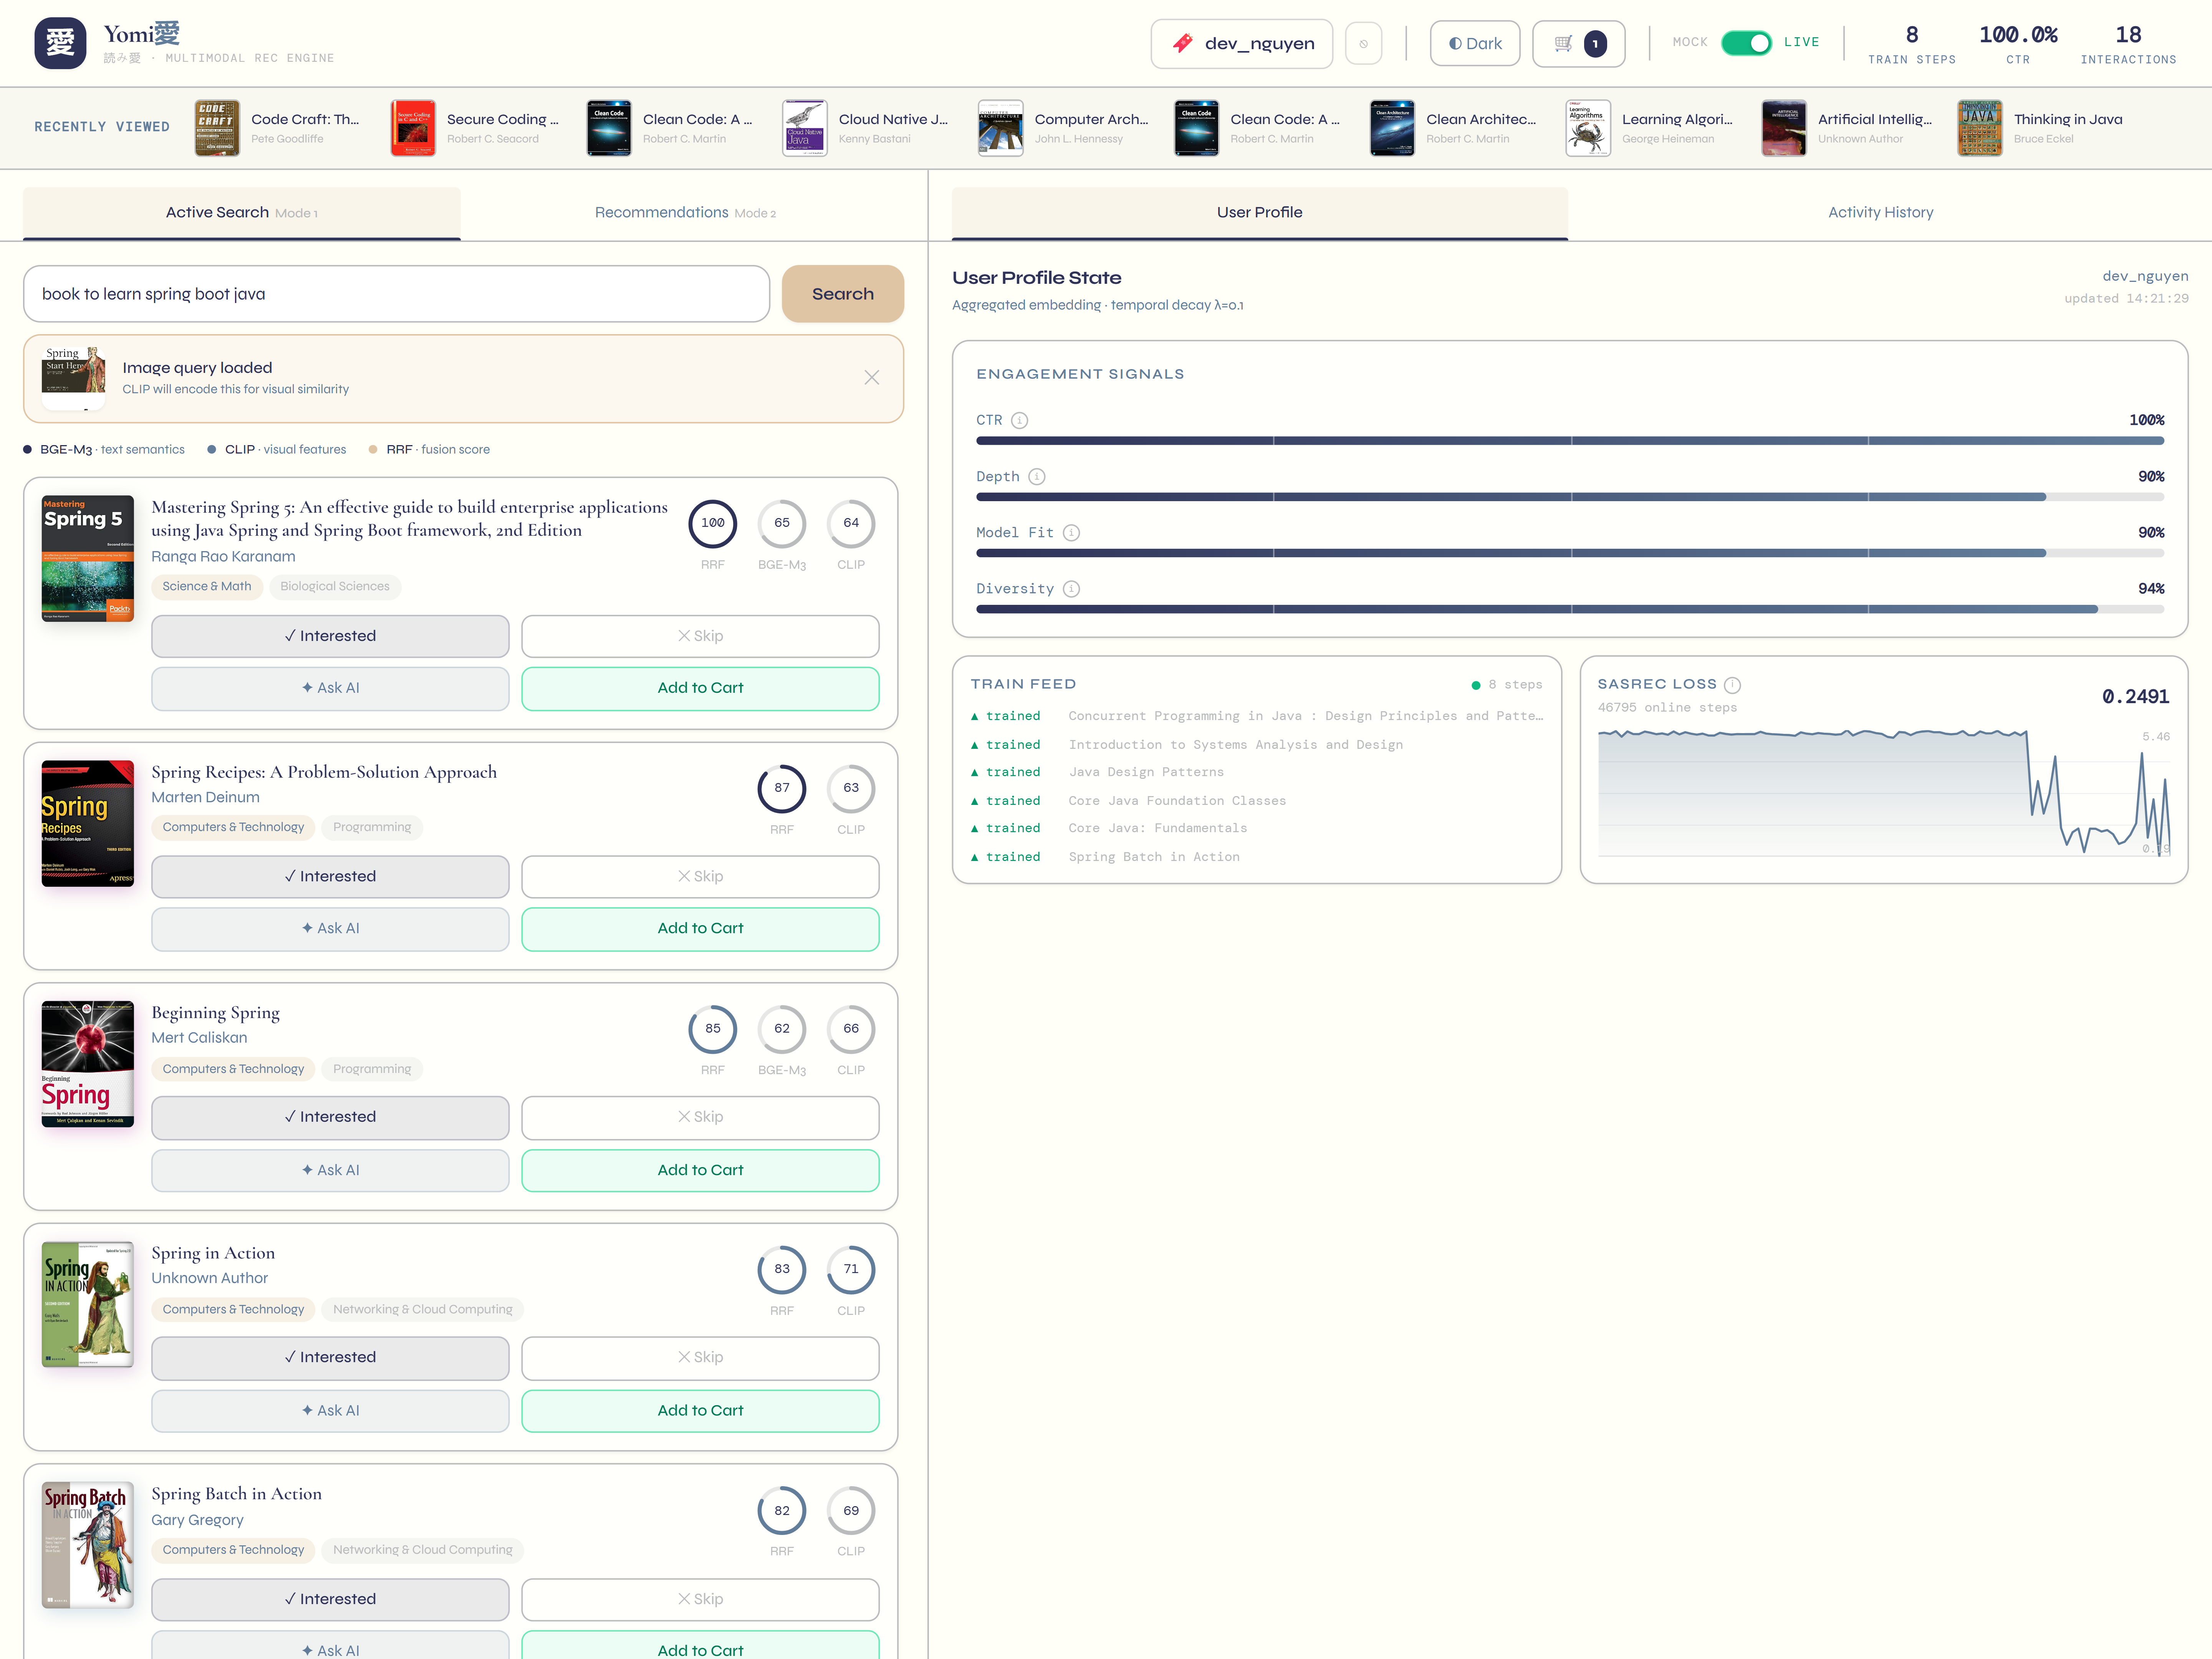
\includegraphics[width=0.92\textwidth]{images/chapter6/fig_app_interface}
\caption{Main application interface. The header contains user controls, the Mock/Live toggle, session statistics (Train Steps, CTR, Interactions), and the Recently Viewed strip. The left panel (42\% width) holds the Active Search and Recommendations tabs. The right panel holds the User Profile and Activity History tabs.}
\label{fig:app_interface}
\end{figure}

\subsection{Login Gate}

Before the main interface loads, a full-screen login page is presented.
The user types a user ID (no password is required) and submits the form.
The frontend calls \texttt{POST /auth/check}: if the ID exists in MongoDB the session begins immediately; if not, the user is prompted to confirm creation via \texttt{POST /auth/create}.
A \textit{Continue as Guest} button assigns a randomly generated \texttt{guest\_XXXXXX} identifier that bypasses the MongoDB lookup.
Guest sessions receive the full search experience but are excluded from personalised recommendations and Cleora graph updates.
The resolved user ID is written to \texttt{localStorage} so that returning users skip the gate on subsequent visits.

\subsection{Header}

The header contains five areas.
The \textbf{brand area} displays the application logotype and subtitle.
The \textbf{user badge} shows the active user ID and a sign-out button.
The \textbf{controls area} provides a dark/light mode toggle and a shopping cart button displaying the current item count.
The \textbf{Mock/Live toggle} switches the frontend between the live FastAPI backend and built-in mock data; a toast notification confirms every mode change.
The \textbf{stats counters} display three live session metrics: \textit{Train Steps} (number of DIF-SASRec gradient steps), \textit{CTR} (click-through rate), and \textit{Interactions} (total event count).
Below the main row, a \textit{Recently Viewed} strip shows cover thumbnails and titles for the user's most recent interactions, sourced from the \texttt{GET /profile} response in live mode.

\subsection{Left Panel — Active Search (Mode 1)}
\label{sec:app_search_panel}

The left panel (42\% of viewport width) has two tabs: \textit{Active Search} and \textit{Recommendations}.

The \textit{Active Search} tab contains a text input field, a search button, and an image drop zone.
When an image file is loaded, the drop zone transitions from a dashed placeholder to a thumbnail preview confirming that the CLIP encoder will process it; the image can be cleared via a dismiss button.
An encoder legend below the input shows the three retrieval signals: BGE-M3 (text semantics), CLIP (visual features), and RRF (fusion score).
While a search request is in flight, four animated skeleton placeholder cards occupy the result area.
On response arrival, each result is rendered as a card containing the cover image, title, author, genre tag(s), and relevance score badges.
An RRF badge is present on every card; a BGE-M3 badge appears when a text query is active and a CLIP badge appears when an image is active, so that up to three badges are shown for a combined text-and-image query.
Each card provides four interaction controls: \textit{Interested} (logs a click), \textit{Skip} (logs a skip), \textit{Ask AI} (opens a streaming book-description popover), and \textit{Add to Cart} (logs a cart event).

\subsection{Left Panel — Recommendations (Mode 2)}
\label{sec:app_rec_panel}

The \textit{Recommendations} tab displays a mode status pill, a manual refresh button with a last-updated timestamp, and two sub-tabs.
The \textit{People Also Buy} sub-tab renders Pipeline~A output (Cleora co-purchase neighbours re-ranked by the user's BGE-M3 profile vector).
The \textit{You Might Like} sub-tab renders Pipeline~B output (DIF-SASRec sequential recommendations).
When \textit{You Might Like} is active and the user is in personalised mode, a horizontal input-sequence strip is displayed above the recommendation cards.
This strip shows the user's most recent click and cart interactions — up to eight items — in chronological order, representing the exact sequence that DIF-SASRec reads when generating the next-item prediction.
Each recommendation card carries a coloured pipeline layer tag and score badges.
People Also Buy cards (Pipeline~A) display BGE-M3 and CLIP cosine-similarity badges reflecting the alignment between the user's profile vector and the candidate item; the layer tag reads \textit{Cleora~+~BGE-M3} or \textit{Cleora~+~CLIP} depending on which signal was dominant.
You Might Like cards (Pipeline~B) display a normalised SASRec intent score, scaled so that the top-ranked candidate receives 1.0 and the remaining candidates are proportional to their actual dot-product gap; the layer tag reads \textit{DIF-SASRec}.
Items that are new since the previous refresh are highlighted for four seconds.

\subsection{Right Panel — User Profile and Activity History}
\label{sec:app_profile_panel}

The right panel contains two tabs: \textit{User Profile} and \textit{Activity History}.

The \textit{User Profile} tab is arranged as a grid of three cards.
The \textbf{Engagement Signals} card (full width) renders a \texttt{ProfileRadar} radar chart visualising five dimensions derived from the session's interaction history: click rate, cart rate, skip rate, interaction count, and recency.
The \textbf{Train Feed} card lists the six most recent interactions with per-event outcome labels (\textit{trained} for clicks and carts, \textit{skipped} for skips) alongside a gradient-step counter.
The \textbf{SASRec Loss} card renders an SVG sparkline of the full training loss history as a filled area chart.
A dashed divider marks the boundary between the pretraining phase and the online fine-tuning phase; an information tooltip beside the chart title explains the expected loss-scale drop between the two phases.
When a gradient step fires, a transient loss-decrease badge is displayed for 2.5 seconds beside the current loss value, providing immediate confirmation that the model has updated.

The \textit{Activity History} tab displays a scrollable chronological list of all in-session interactions, each showing the book cover, title, author, action type, and a timestamp precise to the second.
